\documentclass[a4paper,kulak]{kulakarticle}

\usepackage[utf8]{inputenc}
\usepackage[dutch]{babel}
\usepackage[]{amsmath}
\usepackage{float}
\usepackage{subcaption}
\usepackage{graphicx,wrapfig,lipsum}

\date{Academiejaar 2018-2019}
\address{
  Informatica \\
  Statistische modellen en data-analyse \\
  Prof. Stefan Van Aelst \& Stijn Rebry}
\title{Verslag project 1}
\author{Thomas Bamelis R0640219 \& Michiel Jonckheere R0665594}

\begin{document}

\maketitle

\tableofcontents
\newpage
\section*{Introductie}
In dit verslag wordt nagegaan hoe de oorzaken van overlijden verschillen tussen landen en regio's in
de wereld. Er zijn schattingen van het aantal overlijdens beschikbaar voor 183 landen,
opgesplitst naar 32 verschillende doodsoorzaken. De landen worden gegroepeerd in 6 groepen volgens
geografische ligging en 2 groepen naargelang de globale ontwikkeling van het betreffende land. De gegevens
met betrekking tot de doodsoorzaken zijn afkomstig van de Wereldgezondheidsorganisatie \cite{ghe} en betreffen
het jaar 2016, de indeling in groepen is deze volgens de Verenigde Naties \cite{vn}. 
Deze gegevens werden verwerkt en geïnterpreteerd als proporties van de soorten sterfgevallen per land.

\section{Clustering}
Als eerste werd een cluster-analyse uitgevoerd op de gegevens. Eerst bespreken we de gegevens zonder schalen, daarna met.
\subsection{Zonder schalen}
Om een idee te krijgen van hoeveel clusters er best worden genomen, werden het agglomerate nesting algoritme en divisive analysis toegepast.
Agglomerate nesting werd gedaan met de volgende dissimilariteiten: group average, nearest neighbour en furthest neighbour, in die volgorde met daarna divisive analysis.
Zie figuren \ref{fig:hcnd} op p\pageref{fig:hcnd} en \ref{fig:hcnb} op p\pageref{fig:hcnb} in de bijlage \ref{b}.
Gegeven deze figuren lijkt het meest aannemelijk om 2, 4 en 6 klassen te proberen.
De gebruikte clustering algoritmes zijn in volgorde k-means, partitioning around mediods en fuzzy analysis.
De clustering ermee voor 2, 4 en 6 klassen werd geëvalueerd via een silhouette plot en een clusplot.
Zie figuur \ref{fig:cne} op p\pageref{fig:cne}.
Hieruit blijkt dat partitioning around mediods met 2 clusters het beste presteert met een silhouette coëfficiënt van 0.50 (cluster 1 : 0.69 en cluster 2 : 0.43).
Dit is niet bepaald goed en balanceert op het randje van een zwakke structuur.
\subsection{Met schalen}
 We trekken hierbij dezelfde conclusies omtrent het aantal klassen, 2, 4, en 6.
 Zie figuren \ref{fig:hcd} op p\pageref{fig:hcd}en \ref{fig:hcb} op p\pageref{fig:hcb}.
 Na dezelfde clustering algoritmes toegepast te hebben (figuur \ref{fig:ce} op p\pageref{fig:ce}), is de best geobserveerde silhouette coëfficiënt 0.23.
 Hieruit besluiten we dat clustering met schalen aanzienlijk slechter is dan zonder schalen.
 We besluiten dus verder te werken met het beste resultaat zonder schalen.
\subsection{Beschrijving clusters}
We bekijken nu nader de twee clusters geselecteerd door pam met twee clusters zonder schalen.
We bekijken eerst hoeveel landen uit een bepaalde regio in een bepaalde cluster zitten.
\begin{table}[ht]
\centering
\begin{tabular}{rrrrrr}
  \hline
 Cluster & Africa & America & Asia & Europe & Oceania \\ 
  \hline
1 &  45 &   0 &   2 &   0 &   1 \\ 
  2 &   9 &  33 &  44 &  40 &   9 \\ 
   \hline
\end{tabular}
\end{table}

Hieruit kunnen we afleiden dat 45 van de 48 landen in de eerste cluster Afrikaanse landen zijn.
Cluster twee bevat bijna alle landen uit America, Asia, Europe en Oceania.
Ze bevat ook nog 9 Afrikaanse landen.
De eerste cluster neem dus 4/5 van de Afrikaanse landen en op 3 landen na.
Het clustering algoritme vindt dus vooral onderscheid tussen Afrikaanse landen tegenover de rest van de wereld qua doodsoorzaken.

\begin{table}[ht]
\centering
\begin{tabular}{rrrrr}
  \hline
 Cluster & \#N/B & Developed & Developing & Transition \\
  \hline
1 &   1 &   0 &  47 &   0 \\
  2 &   0 &  36 &  90 &   9 \\
   \hline
\end{tabular}
\end{table}

Clustering tegenover ontwikkeling toont dat de eerste cluster enkel developing landen selecteert, op Congo na waarvan de ontwikkeling onbepaald is.
Het valt echter op dat cluster twee dubbel zoveel developing landen selecteert vergeleken met de eerste cluster, maar ook alle developed en transition landen.
Het is dus niet zo dat de eerste cluster focused op alle developing landen.
Als we dit samen leggen met de region table, kunnen we besluiten dat de eerste cluster hoofdzakelijk Afrikaanse developing landen bevat en de tweede cluster ``de rest''. \newline
Daarnaast kunnen we de verschillen van tussen de clusters bekijken qua doodsoorzaken.
We plotten daarom de marginale gemiddelden van de eerste cluster, afgetrokken met de marginale gemiddelden van de tweede cluster.
Zie figuur \ref{fig:dm} op p\pageref{fig:dm}.
Als we de drie hoofdcategoriën van doodsoorzaken bekijken (de verschillende kleuren), blijkt dat communicable, maternal, perinatal and nutritional conditions meer voorkomen bij de eerste cluster dan bij de tweede.
We zien ook dat twee noncommunicable diseases aanzienlijk meer voorkomen in de tweede cluster, met nog eens 5 van die doodsoorzaken licht meer voorkomen in de tweede cluster.
Over de injuries tussen de twee clusters valt niets significants te zeggen. \newline
Met dit alles samen kunnen we besluiten dat de meeste Afrikaanse landen die developing zijn een proportioneel opvallend hoger aantal  communicable, maternal, perinatal and nutritional conditions bevatten en een proportioneel lager aantal noncommunicable diseases hebben tegenover de rest van de wereld.


\section{Principaalcomponentenanalyse}
Voor de principaalcomponentenanalyse wordt enkel gekeken naar de niet geschaalde gegevens. Dit zagen we al in de vorige sectie dat de geschaalde gegevens voor minder goede resultaten zorgden. Om voor de principaalcomponenten toch zeker te zijn dat de niet geschaalde gegevens hiervoor ook beter zijn, werd toch eens een vergelijking gedaan. In tabel \ref{table:pcaScaledVSNot} is deze vergelijking te zien. De eerste zes principaalcomponenten van de originele data verklaren ongeveer 95\% van de variantie van de data. Bij de geschaalde gegevens verklaren de eerste zes slechts 60\% van die variantie. Om aan 95\% te komen zijn er bij de geschaalde data 23 principaalcomponenten nodig. 

\begin{table}[ht]
	\centering
\begin{tabular}{lcccccc}
	\hline 
	& PC1 & PC2 & PC3 & PC4 & PC5 & PC6 \\ 
	\hline 
	Originiele data & 68.9\% & 81.4\% & 86.4\% & 90.4\% & 93.1\% & 95.2\% \\ 
	%\hline 
	Geschaalde data & 29.7\% & 40.4\% & 46.5\% & 52.3\% & 56.5\% & 60.4\%\\ 
	\hline 
\end{tabular} 
\caption{De cumulatieve proportie van de variantie van de eerste zes principaalcomponenten van zowel de originele als de geschaalde data.}
\label{table:pcaScaledVSNot}
\end{table}

We hebben besloten om hier verder te gaan met de eerste vier principaalcomponenten aangezien ze 90\% van de variantie van de data beschrijven. 

\subsection{PC1}
Voor de variarbelen \textit{Malignant Neoplasms} en \textit{Cardiovascular Diseases} vinden we hoge positieve waarden, respectievelijk 0.33 en 0.66. De grootste negatieve waarde voor de eerste principaalcomponent is -0.62 van de variabele \textit{Infections and Parasitic Diseases}. Dit betekent dus bij een hogere PC1 dat er meer doodsoorzaken zijn van \textit{Malignant Neoplasms} en \textit{Cardiovascular Diseases} en minder van \textit{Infections and Parasitic Diseases}. 

Als we dit bekijken voor de landen dan vinden we zeven landen met een lagere PC1 dan de rest. Deze landen zijn \textit{Angola}, \textit{Central African Republic}, \textit{Kenya}, \textit{Lesotho}, \textit{Mozambique}, \textit{South Sudan} en \textit{Zambia}. Wat hier opvalt, is dat deze landen allemaal in Afrika liggen. Als we dan kijken naar de landen met een opvallend hogere PC1 waarde, dan zien we dat merendeel in Europa gelegen is. Om in het algemeen te kijken naar alle landen vergelijken we de landen met een positieve PC1 met de landen met een negatieve. Hieruit vinden we dat er 66\% van de negatieve PC1 waarden uit Afrika komen en 93\% van de positieve waarden komen uit de andere regio's verschillend van Afrika. We kunnen dus uit PC1 Afrika gaan onderscheiden van de andere regio's.

De ontwikkeling afleiden uit PC1 is deels mogelijk. Alle landen die ontwikkeld zijn of in een overgang zitten naar ontwikkeld, hebben allemaal een positieve PC1. Voor de ontwikkelingslanden heeft 50\% een positieve en 50\% een negatieve PC1. Als we dit dan koppelen aan de regio's kunnen we de ontwikkeling gaan afleiden uit de regio waar de negatieve PC1 waarden voorkomen. Dit betekent dus dat een land die in Afrika gelegen is en een negatieve PC1 waarde heeft, hoogstwaarschijnlijk een ontwikkelingsland zal zijn. Landen die in een andere regio dan Afrika liggen en een positieve PC1 hebben, zijn ofwel ontwikkelde landen ofwel overgangslanden. We merken ook op dat de landen in Azi\"e bijna allemaal ontwikkelingslanden zijn. 

\subsection{PC2}
De meest positieve waarden voor PC2 zijn voor de variabelen \textit{Cardiovascular Diseases} en \textit{Infectious and Parasitic Diseases}, met de respectievelijke waarden 0.66 en 0.31. De meest negatieve waarde -0.58 hoort bij de variabele \textit{Malignant Neoplasms}. Dit betekent bij een hogere PC2 waarde dat er minder doden door \textit{Malignant Neoplasms} zijn en juist meer door  \textit{Cardiovascular Diseases} en \textit{Infectious and Parasitic Diseases}. 

Het grootste deel van de landen die een positieve PC2 waarde hebben, zijn landen die in Azi\"e en Afrika liggen. Daar zijn er dus meer doden door \textit{Cardiovascular Diseases} en \textit{Infectious and Parasitic Diseases}. Over de negatieve PC2 waarden zijn er niet echt regio's uit af te leiden. Voornamelijk Amerikaanse en Europese landen hebben het grootste aandeel bij de negatieve waarden en minder opvallend bij de positieve. Wat er ook duidelijk te zien is, is dat er maar een paar Afrikaanse landen een negatieve waarde hebben. Om betere conclusies te trekken, zouden we naar de extremere positieve en negatieve waarden kunnen kijken, maar daarbij valt er nog altijd niets beters te concluderen. 

Voor de ontwikkeling van de landen zien we dat bij een positieve PC2 het grootste deel bij de ontwikkelingslanden zit. Ontwikkelde landen hebben hebben bijna allemaal een negatieve PC2, maar ook 33\% van de ontwikkelingslanden hebben een negatieve PC2. 

We besluiten hieruit dat de positieve PC2 waarden hoogstwaarschijnlijk landen die in Azi\"e of Afrika liggen en ontwikkelingslanden zijn. Bij een negatieve PC2 waarde is de kans het grootst dat het een Amerikaans ontwikkelingsland of een Europees ontwikkeld land is. Als het een Aziatisch land is, dan is dat land een ontwikkelingsland bij een negatieve PC2 waarde.

\subsection{PC3}
Bij PC3 waarden vinden we voor volgende drie verandelijken de meest in het oog springende waarden: \textit{Malignant Neoplasms}, \textit{Infectious and Parasitic Diseases} en \textit{Diabetes Mellitus}. De waarden zijn respectievelijk -0.47, -0.51 en 0.53. Deze principaalcomponent kijk dus naar het verschil tussen de eerste twee en de laatst genoemde variabelen. 

Als we naar de regio's kijken van de landen, zien we dat de lagere PC3 waarden voornamelijk uit de regio's Europa en Afrika komen. De opvallend positieve waarden komen uit de regio's Amerika, Azi\" en Oceani\"e. Voor de ontwikkeling hebben alle ontwikkelde landen een negatieve PC3 waarde, voor de andere waarden is dit wat meer verdeeld en komen extremen in beide gevallen voor. 

\subsection{PC4}
De vierde principaalcomponent vergelijkt de variabele \textit{Diabetes Mellitus} met \textit{Collective Violence and Legal Intervention} en \textit{Neurological Conditions}. De PC4 waarden van deze drie variabelen zijn respectievelijk 0.76, -0.34 en -0.23. 

Bij het kijken naar de regio's en ontwikkeling zien we dat deze over het algemeen rond 0 hangen, al zijn er een paar ontwikkelingslanden die toch relatief grote PC4 waarden hebben. Deze landen zijn twee landen uit Oceani\"e en drie Amerikaanse, nl.  Micronesia en Tonga (eilanden van Oceani\"e) en Antigue en Barbuda, Grenada en Saint Vincent and the Grenadines (allemaal eilanden in de buurt van de Caribische Zee). Op deze eilanden is de PC4 het hoogst en zijn er daar meer doden door \textit{Diabetes Mellitus} en minder door \textit{Collective Violence and Legal Intervention} en \textit{Neurological Conditions}.\\

In figuur \ref{fig:vglPC} staan de plots van de PC1 waarden t.o.v. de PC2, PC3 en PC4 waarden. Hieruit zijn de meest getrokken conclusies ook zichtbaar adhv de kleurtjes en figuurtjes gebruikt voor de verschillende regio's en ontwikkelingen. 

\section*{Besluit}

TODO


\begin{thebibliography}{9}
	
	\bibitem{ghe}
	Global Health Estimates 2016: Deaths by Cause, Age, Sex, by Country and by Region, 2000-2016.
	Geneva, World Health Organization; 2018.
	
	\bibitem{vn}
	Country classification, june 2018. Geneva, United Nations Conference on Trade and Development;
	2018.
	
\end{thebibliography}

\newpage
\section{Bijlage} \label{b}
\subsection{Clustering}
\subsubsection{Zonder schalen}
\begin{figure}[H]
	\centering
	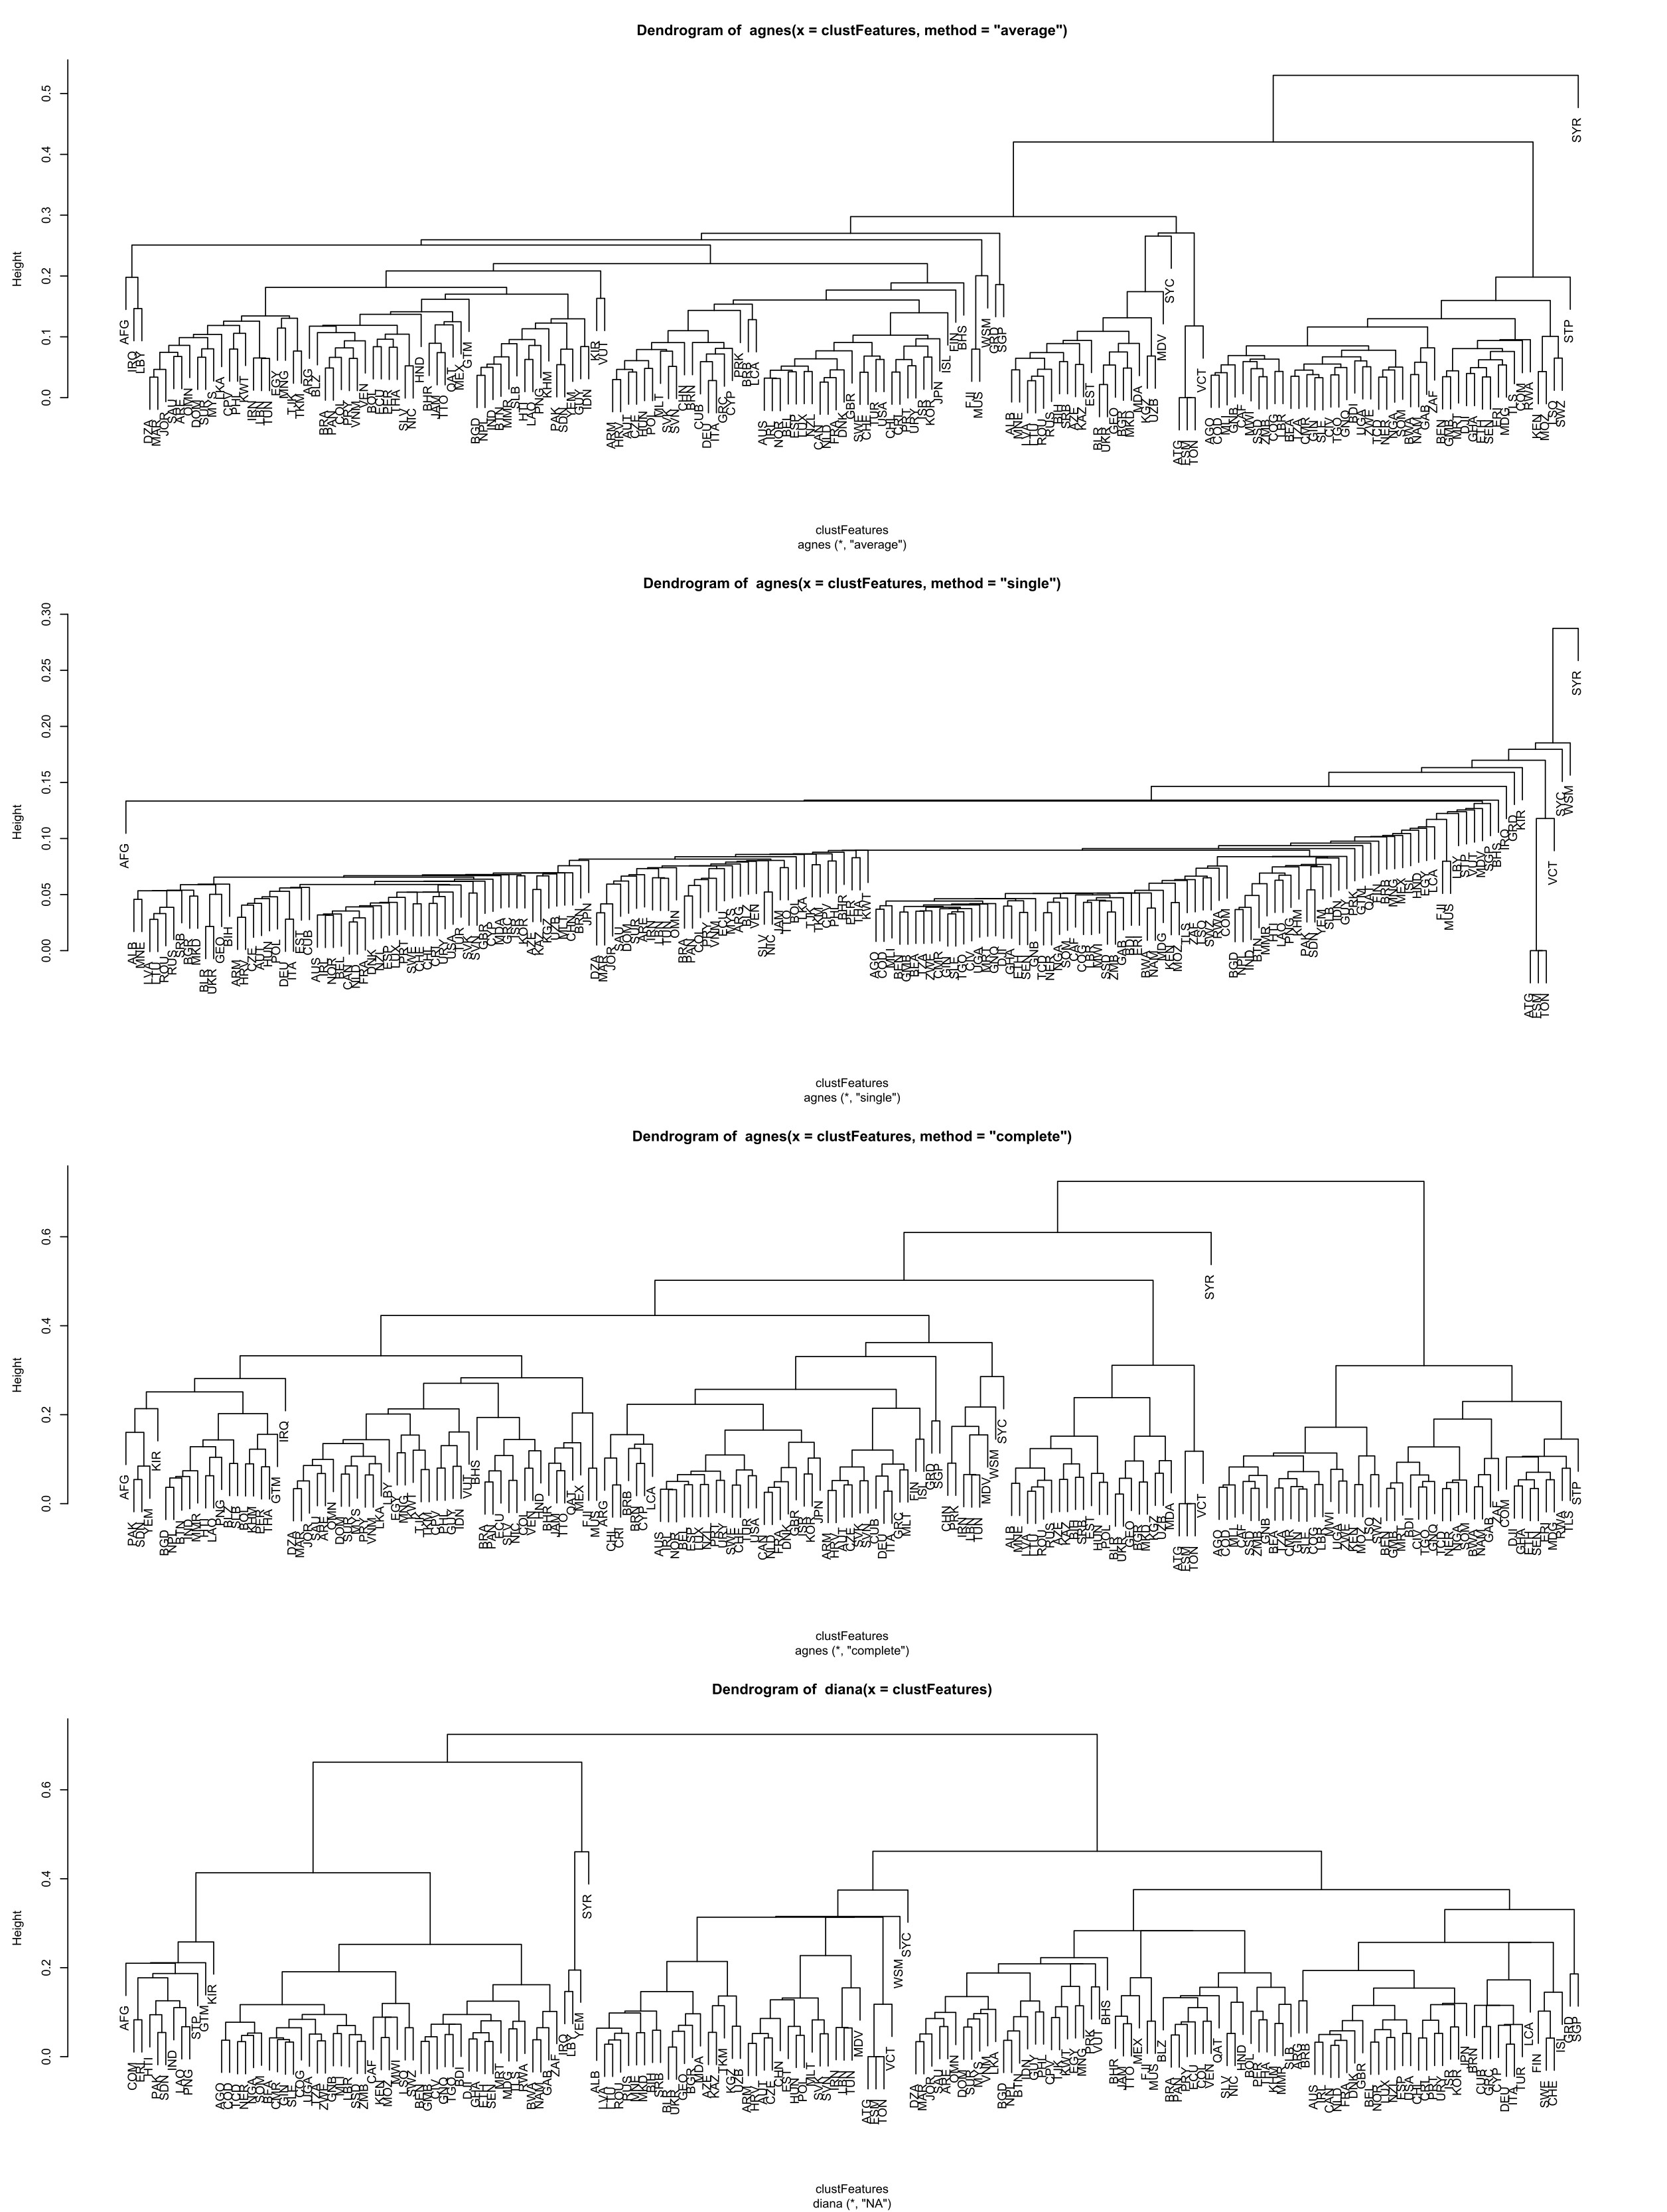
\includegraphics[height=\textheight]{figures/hierachicalClusteringNoScalingDendogram.jpg}
	\caption{Hierchical clustering dendograms}
	\label{fig:hcnd}
\end{figure}
\begin{figure}[H]
	\centering
	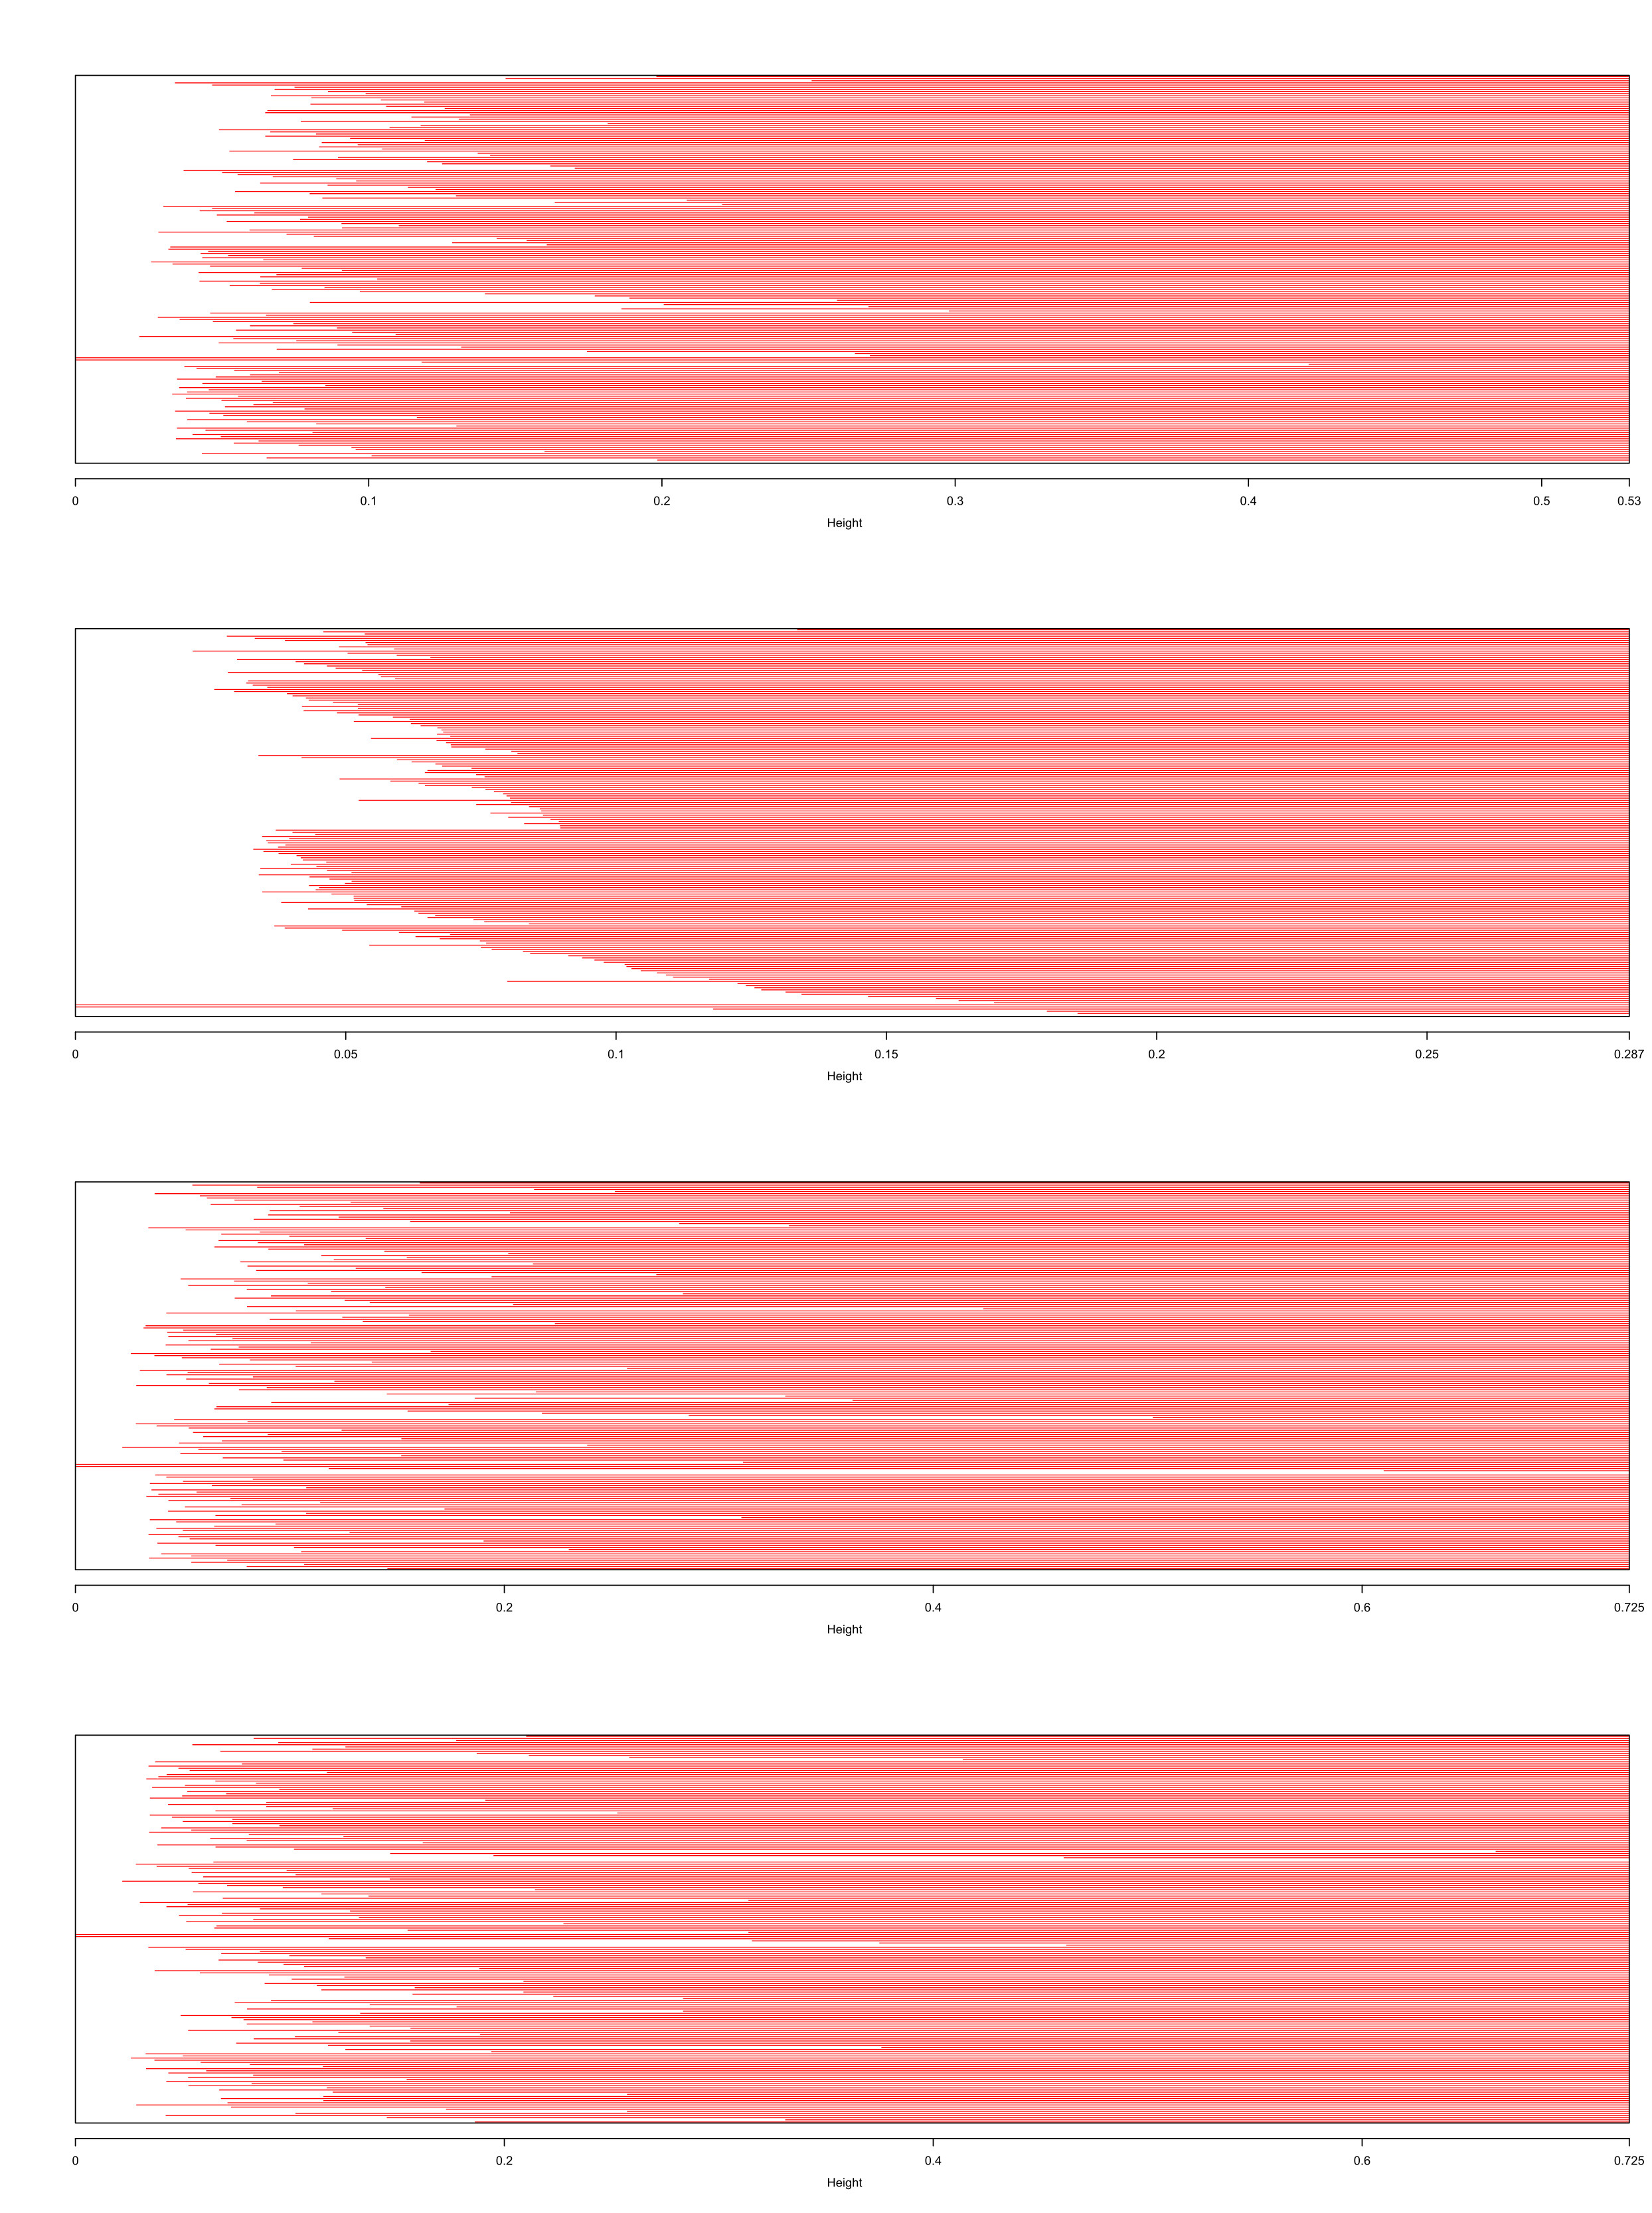
\includegraphics[height=\textheight]{figures/hierachicalClusteringNoScalingBanner.jpg}
	\caption{Hierchical clustering bannerplots}
	\label{fig:hcnb}
\end{figure}
\begin{figure}[H]
	\centering
	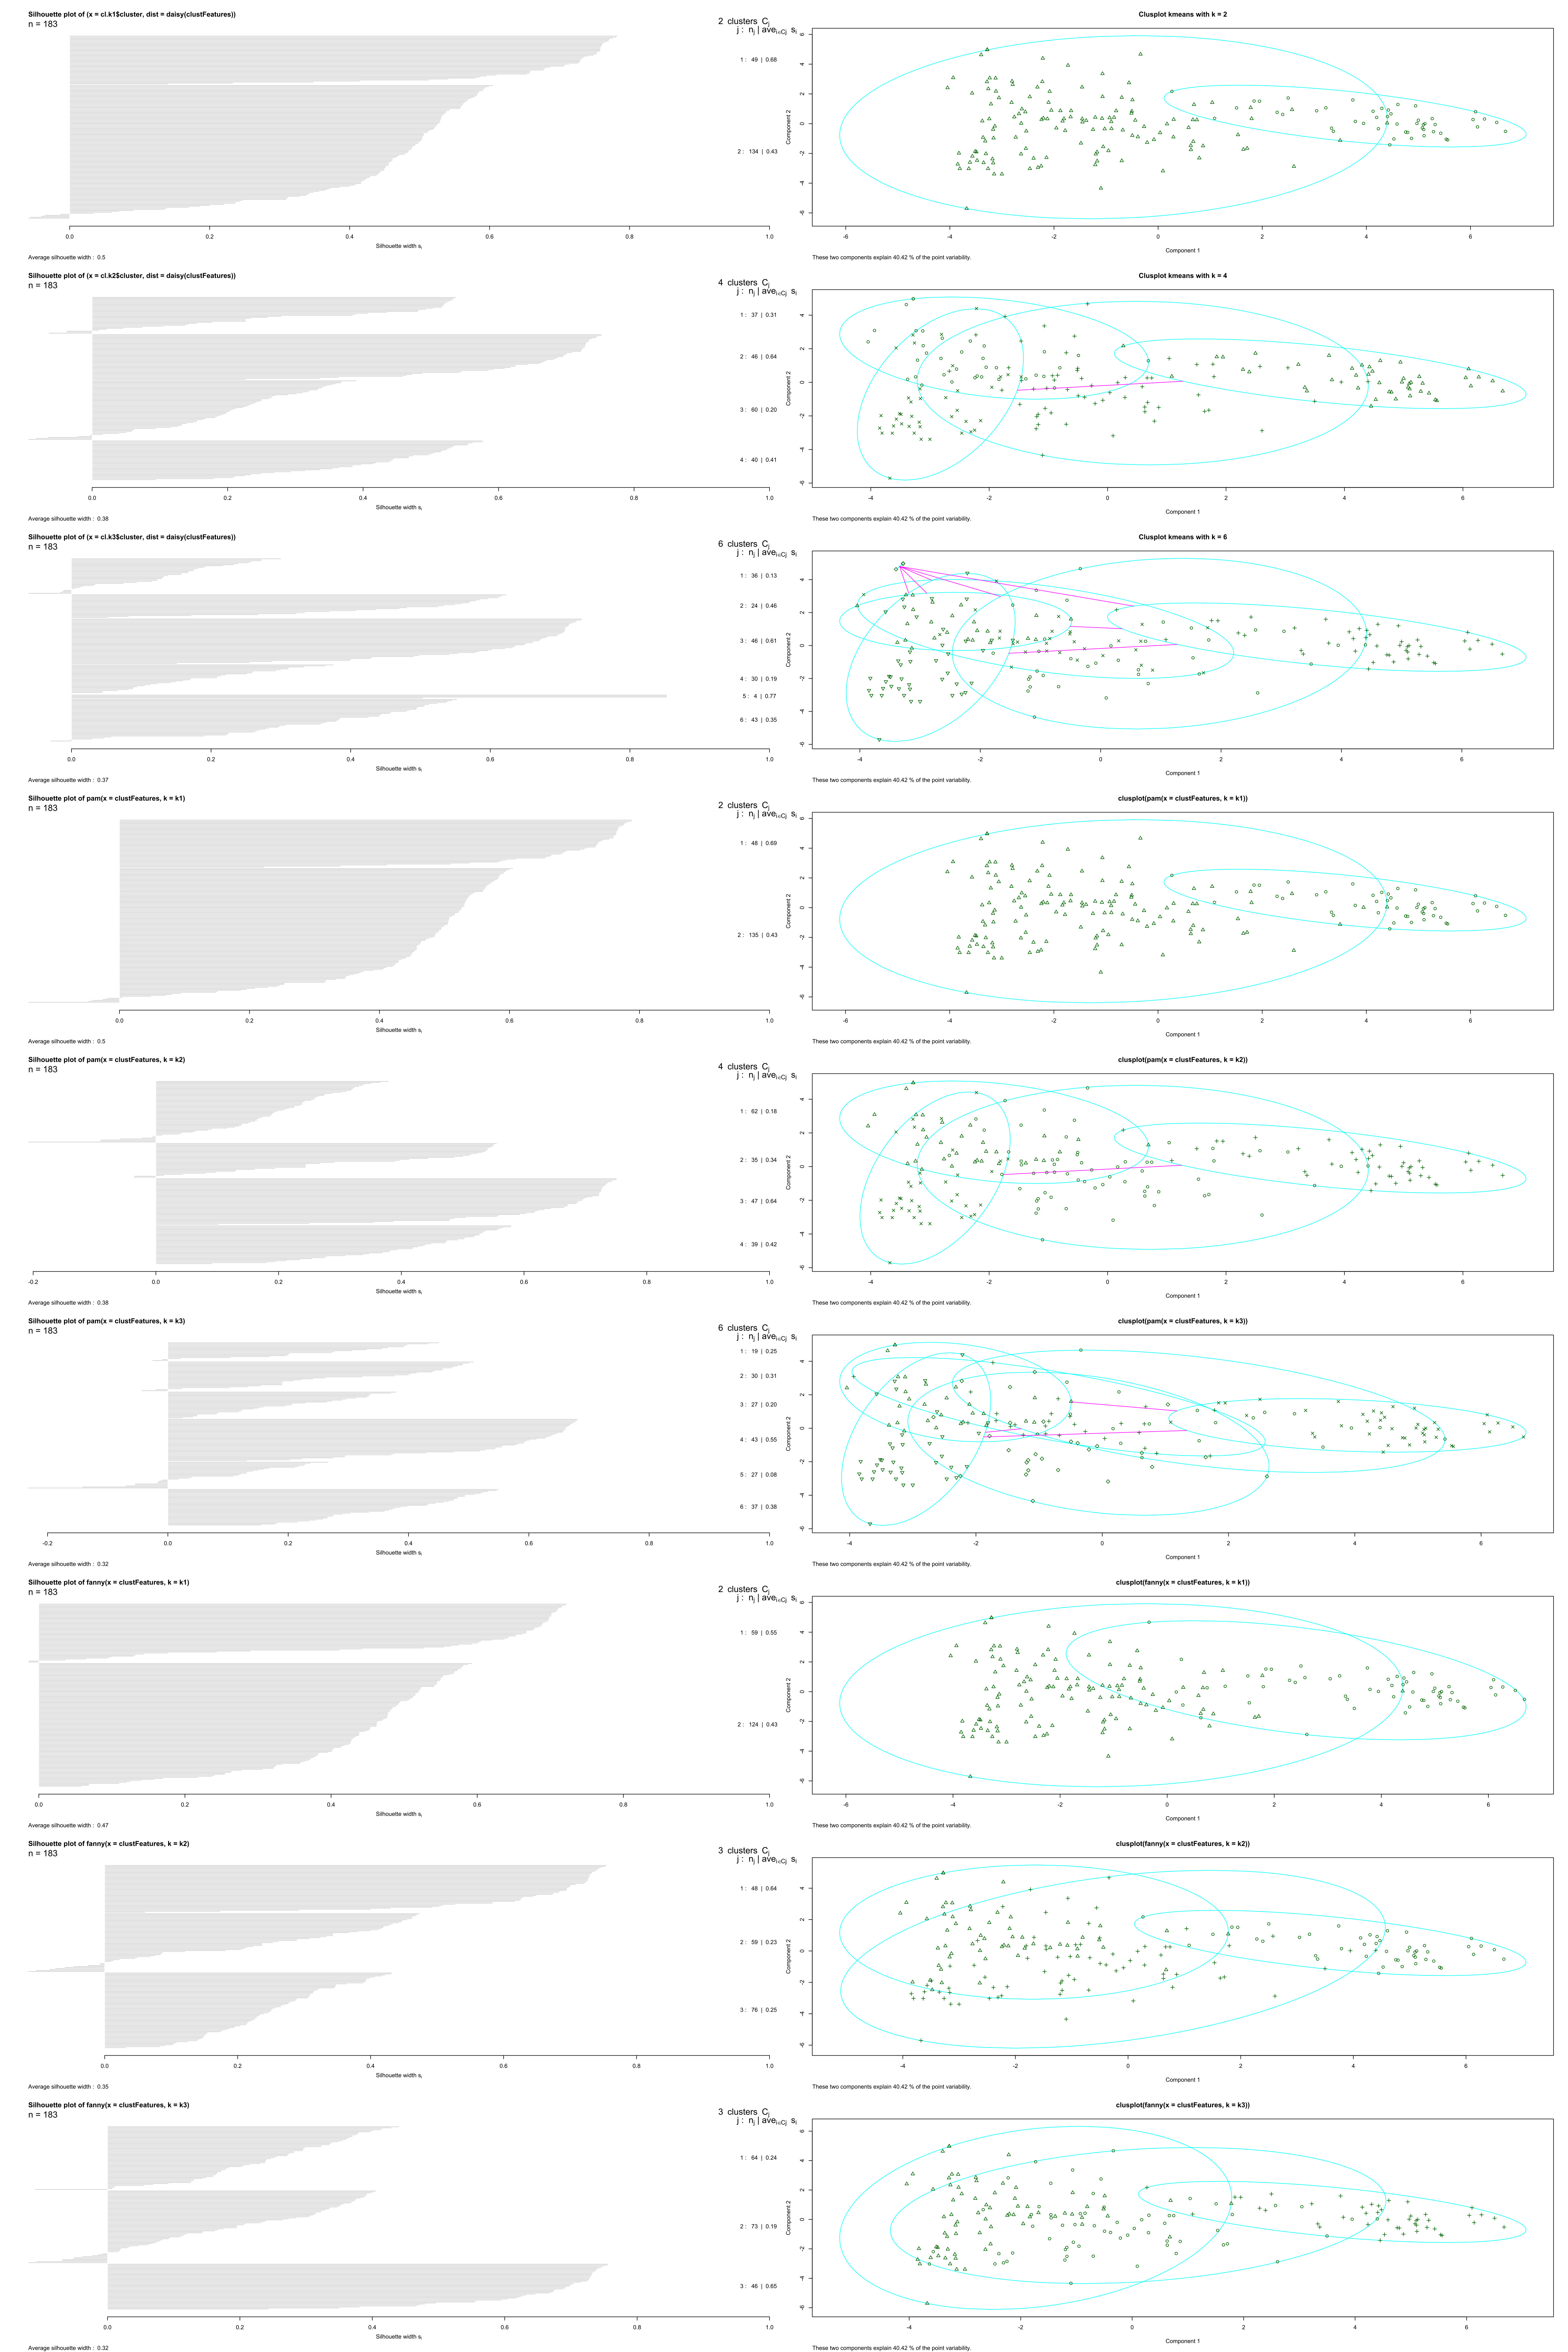
\includegraphics[height=\textheight]{figures/clusteringEvaluationNoScaling.jpg}
	\caption{Clustering evaluatie}
	\label{fig:cne}
\end{figure}
\subsubsection{Met schalen}
\begin{figure}[H]
	\centering
	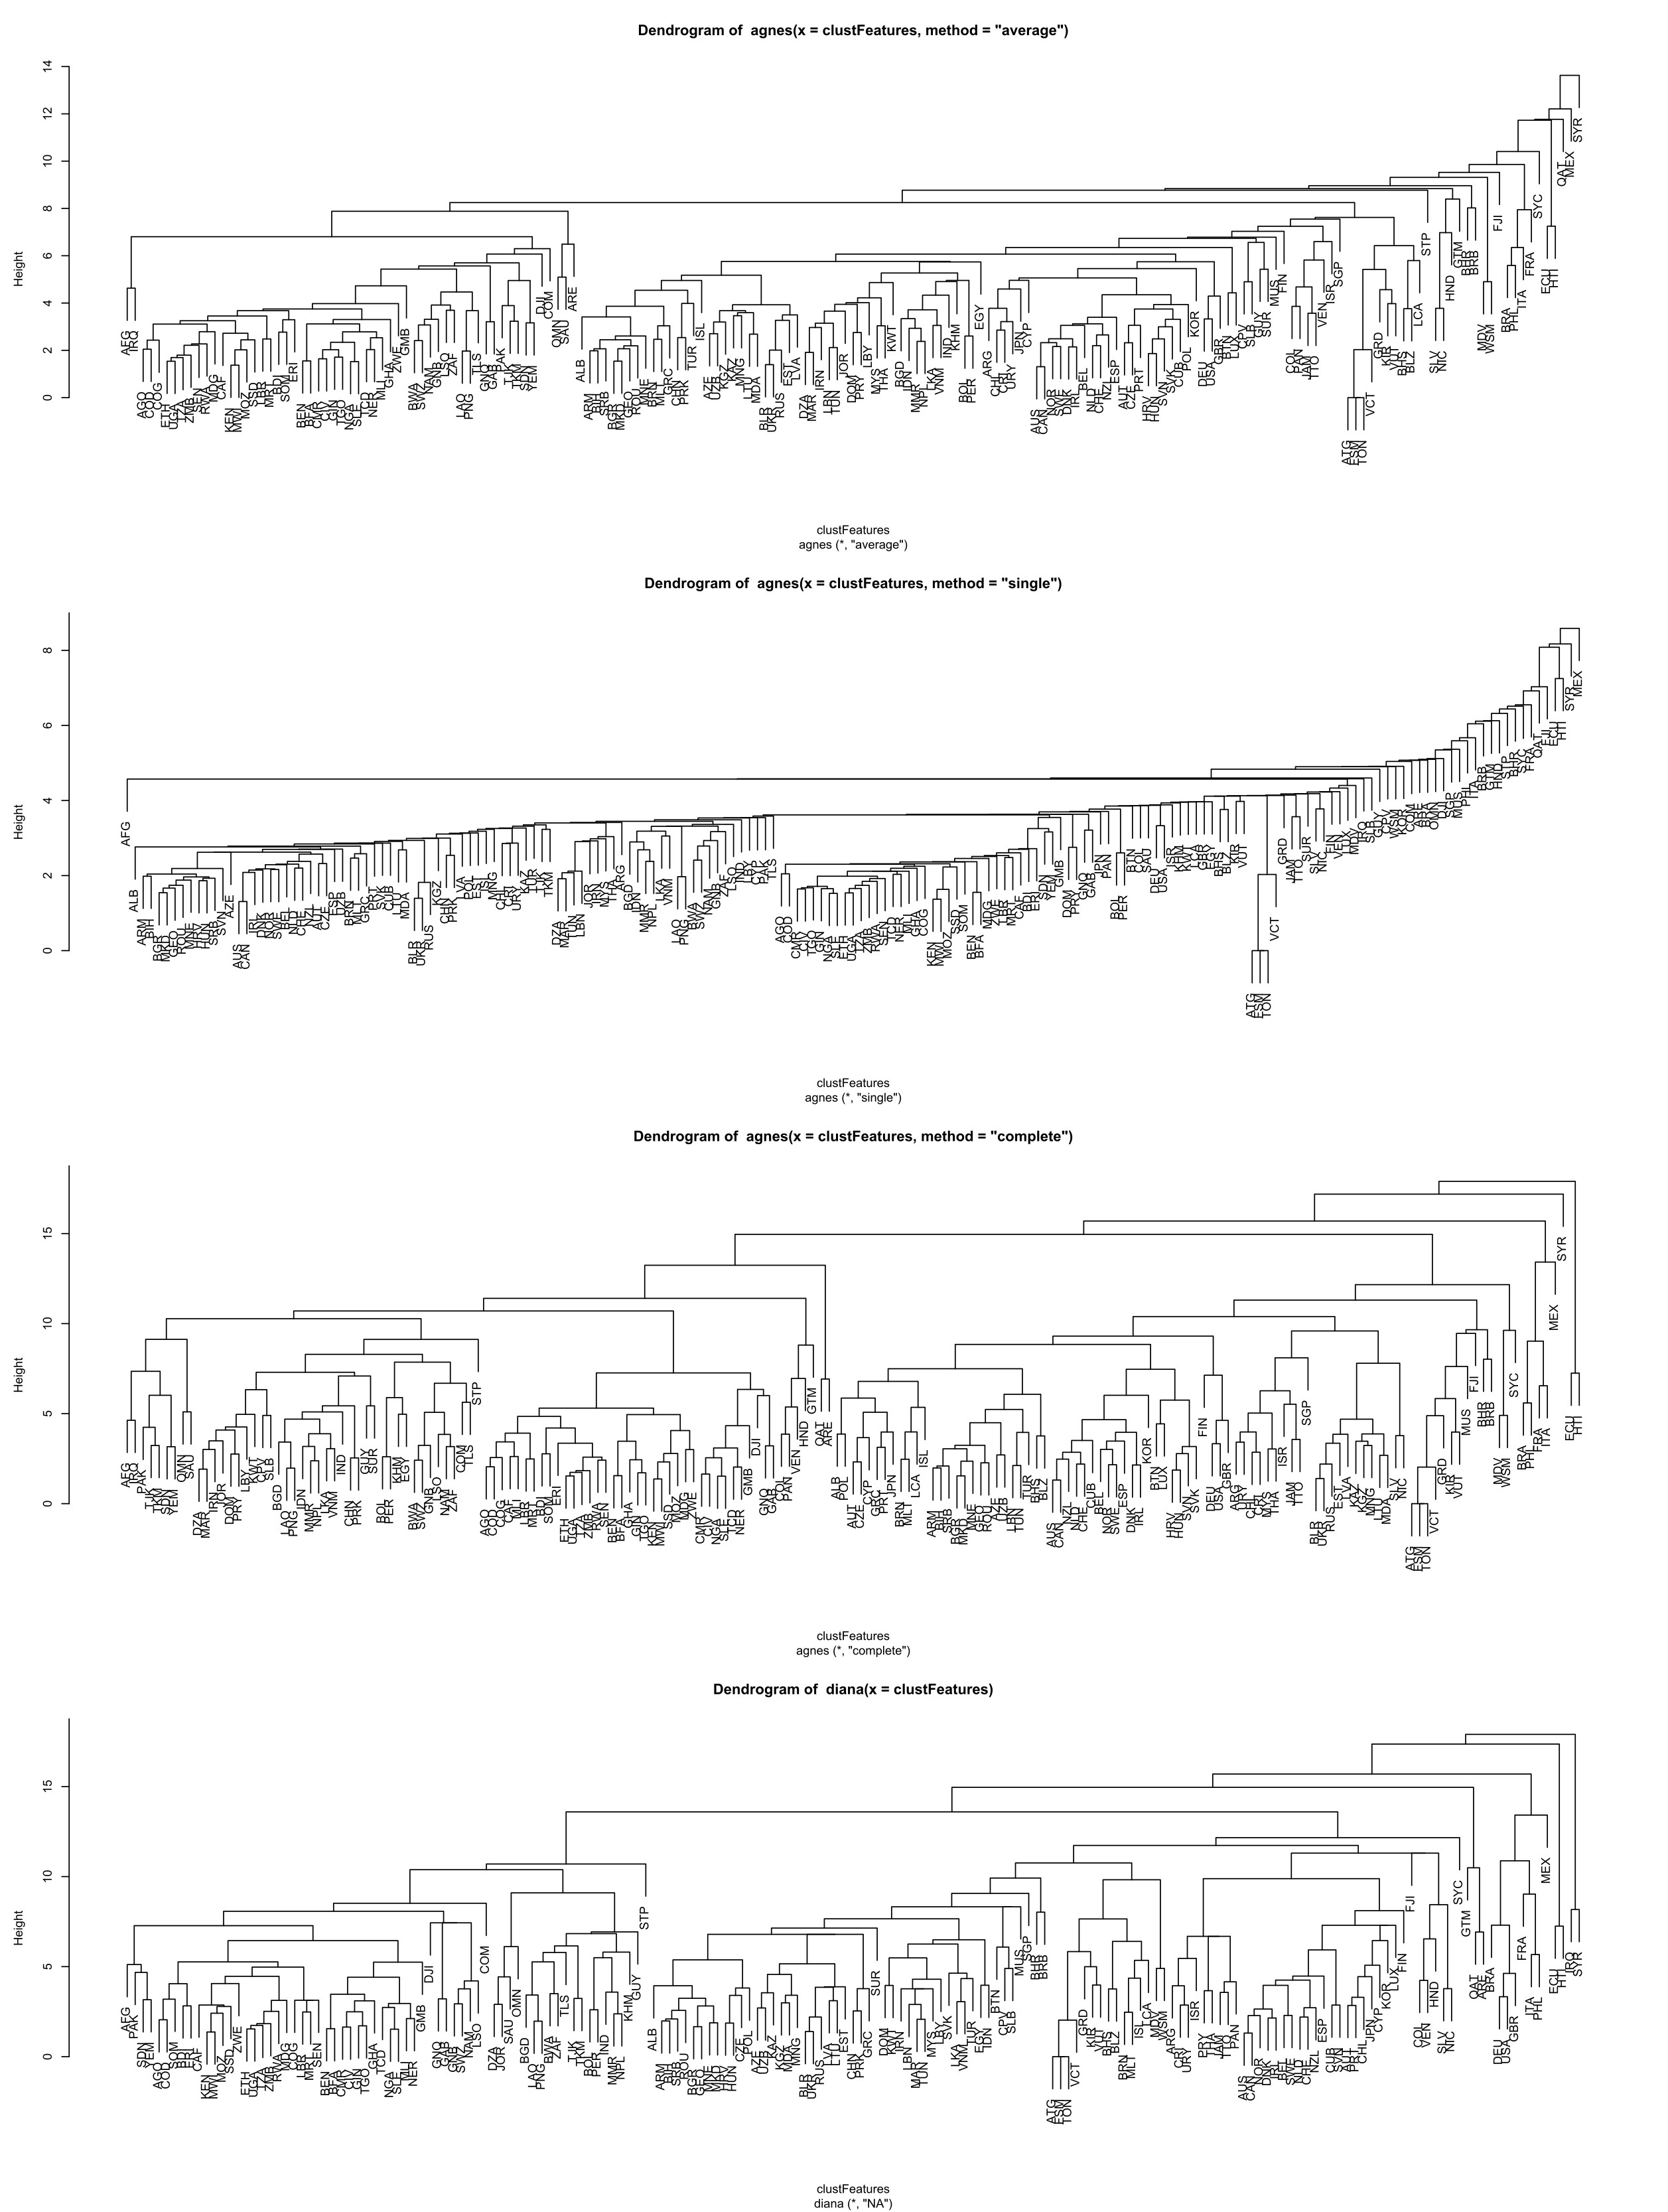
\includegraphics[height=\textheight]{figures/hierachicalClusteringScaledDendogram.jpg}
	\caption{Hierchical clustering dendograms met schalen}
	\label{fig:hcd}
\end{figure}
\begin{figure}[H]
	\centering
	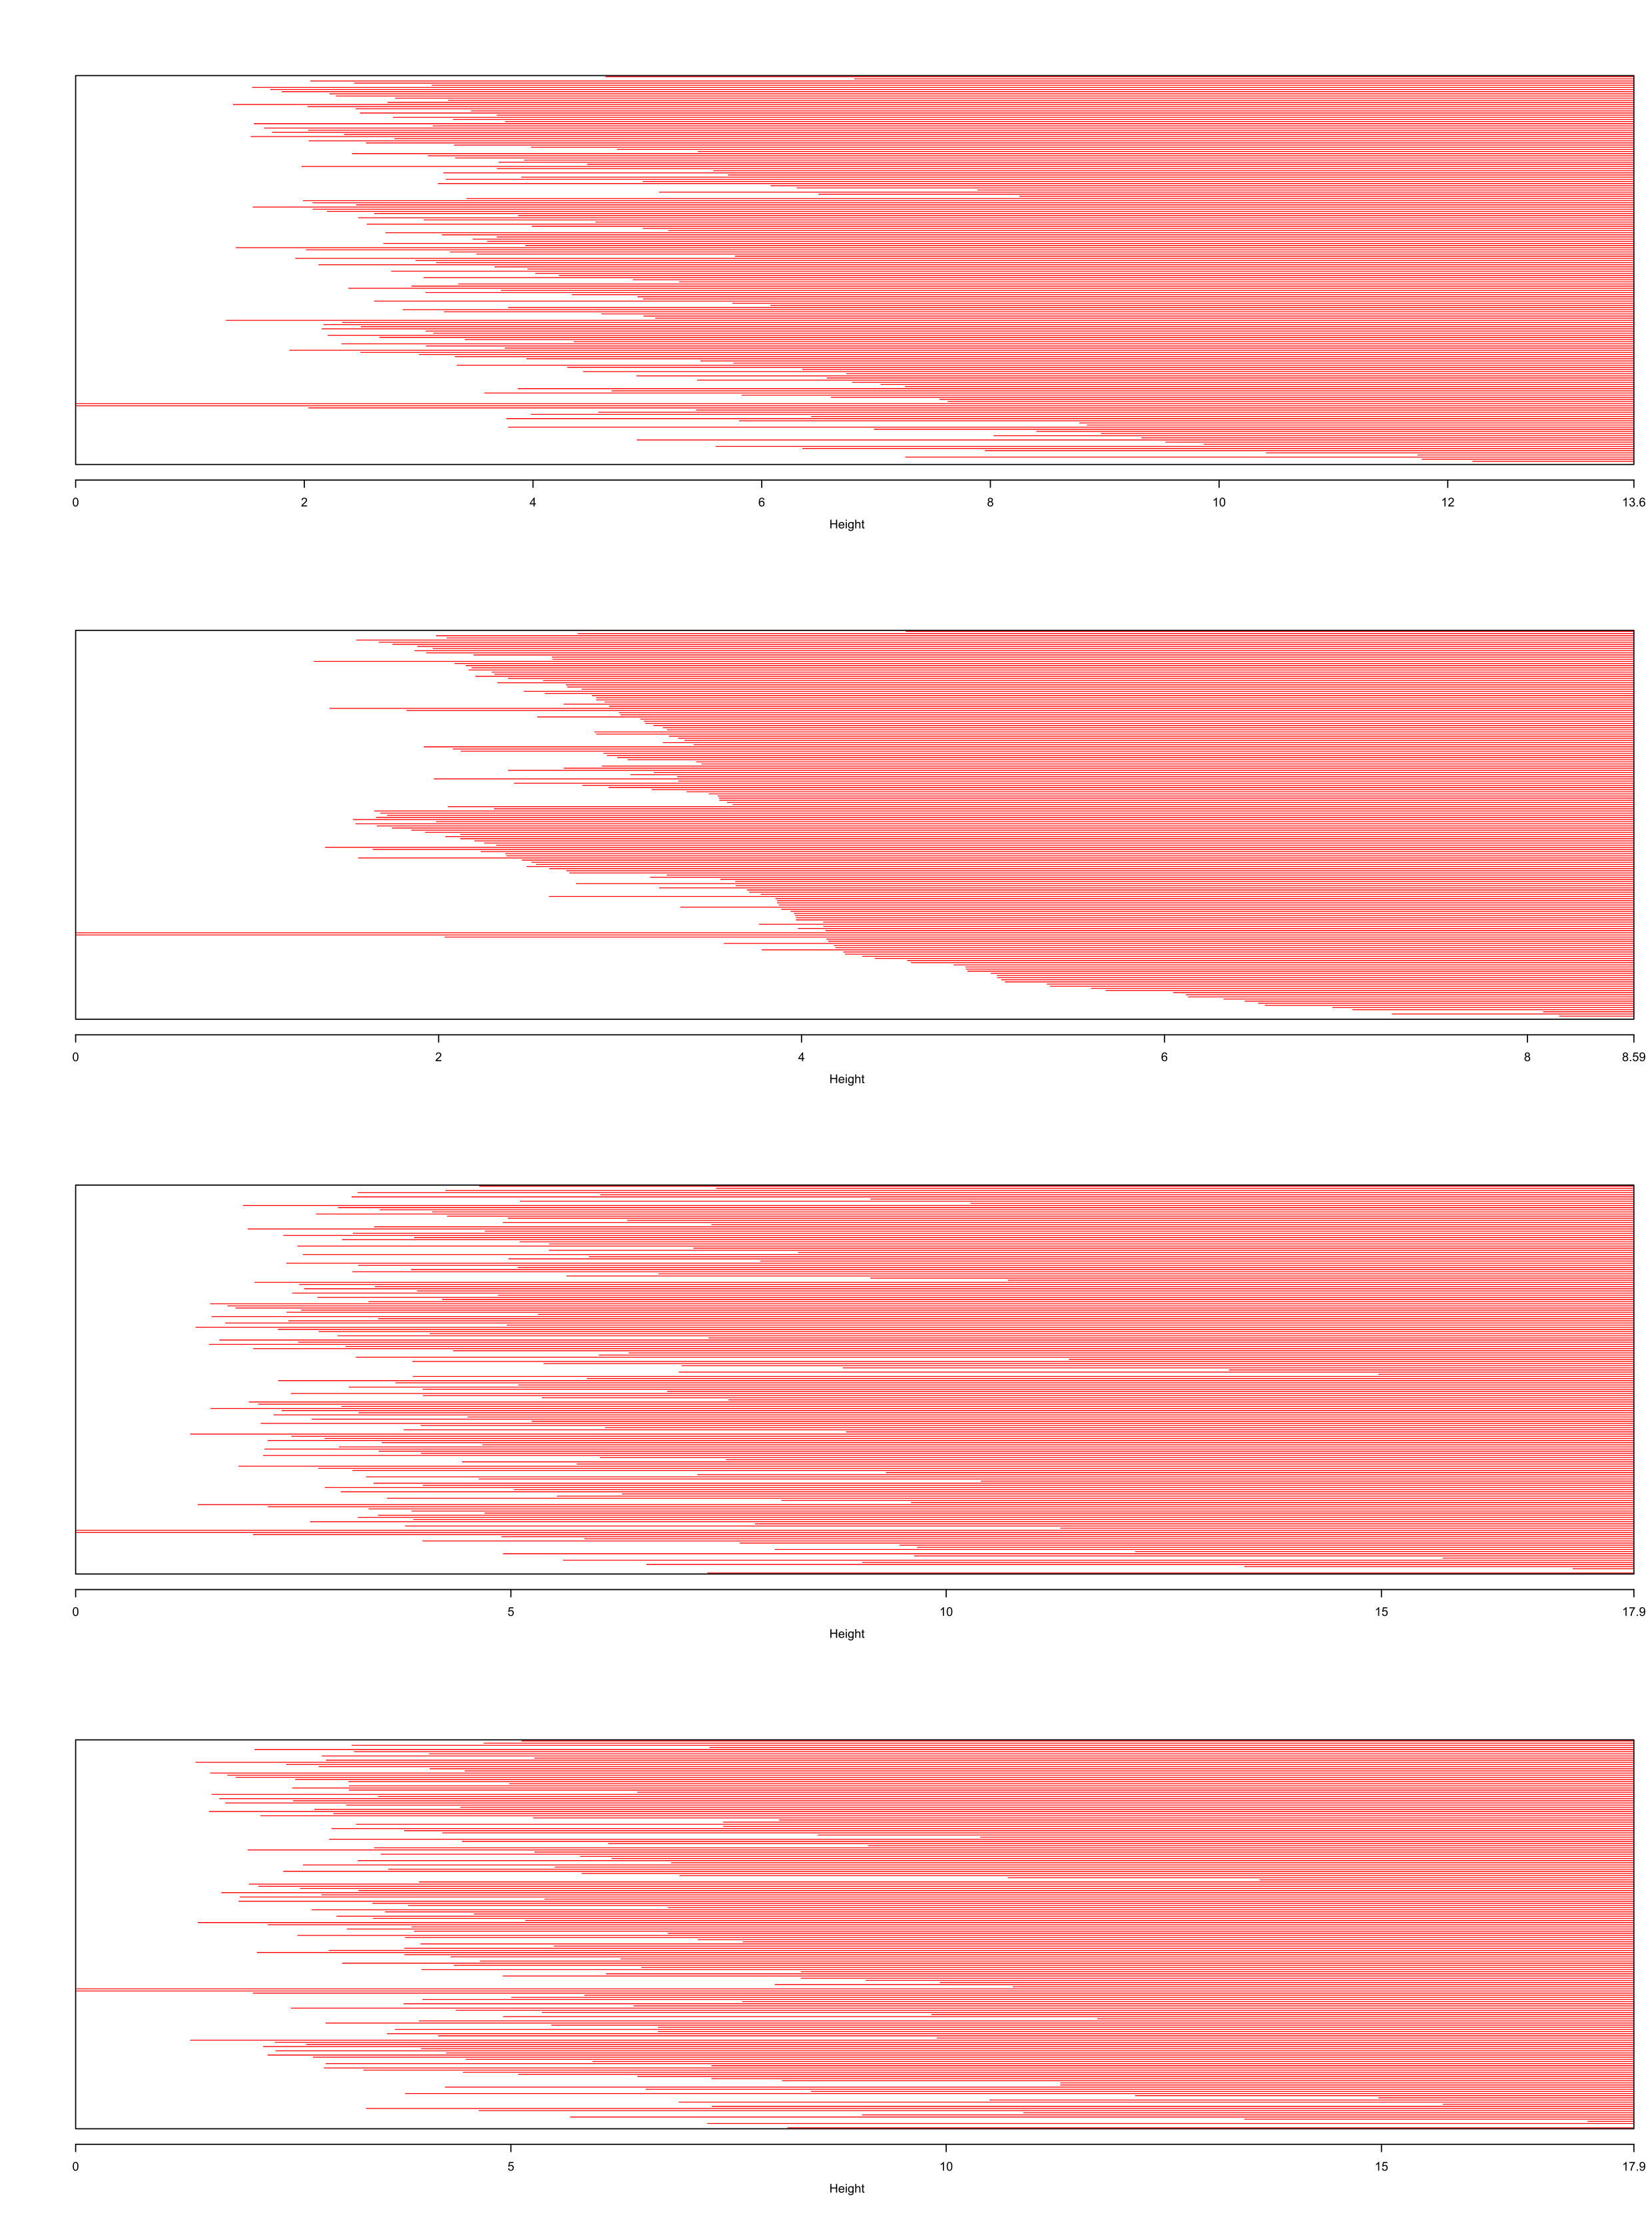
\includegraphics[height=\textheight]{figures/hierachicalClusteringScaledBanner.jpg}
	\caption{Hierchical clustering bannerplots met schalen}
	\label{fig:hcb}
\end{figure}
\begin{figure}[H]
	\centering
	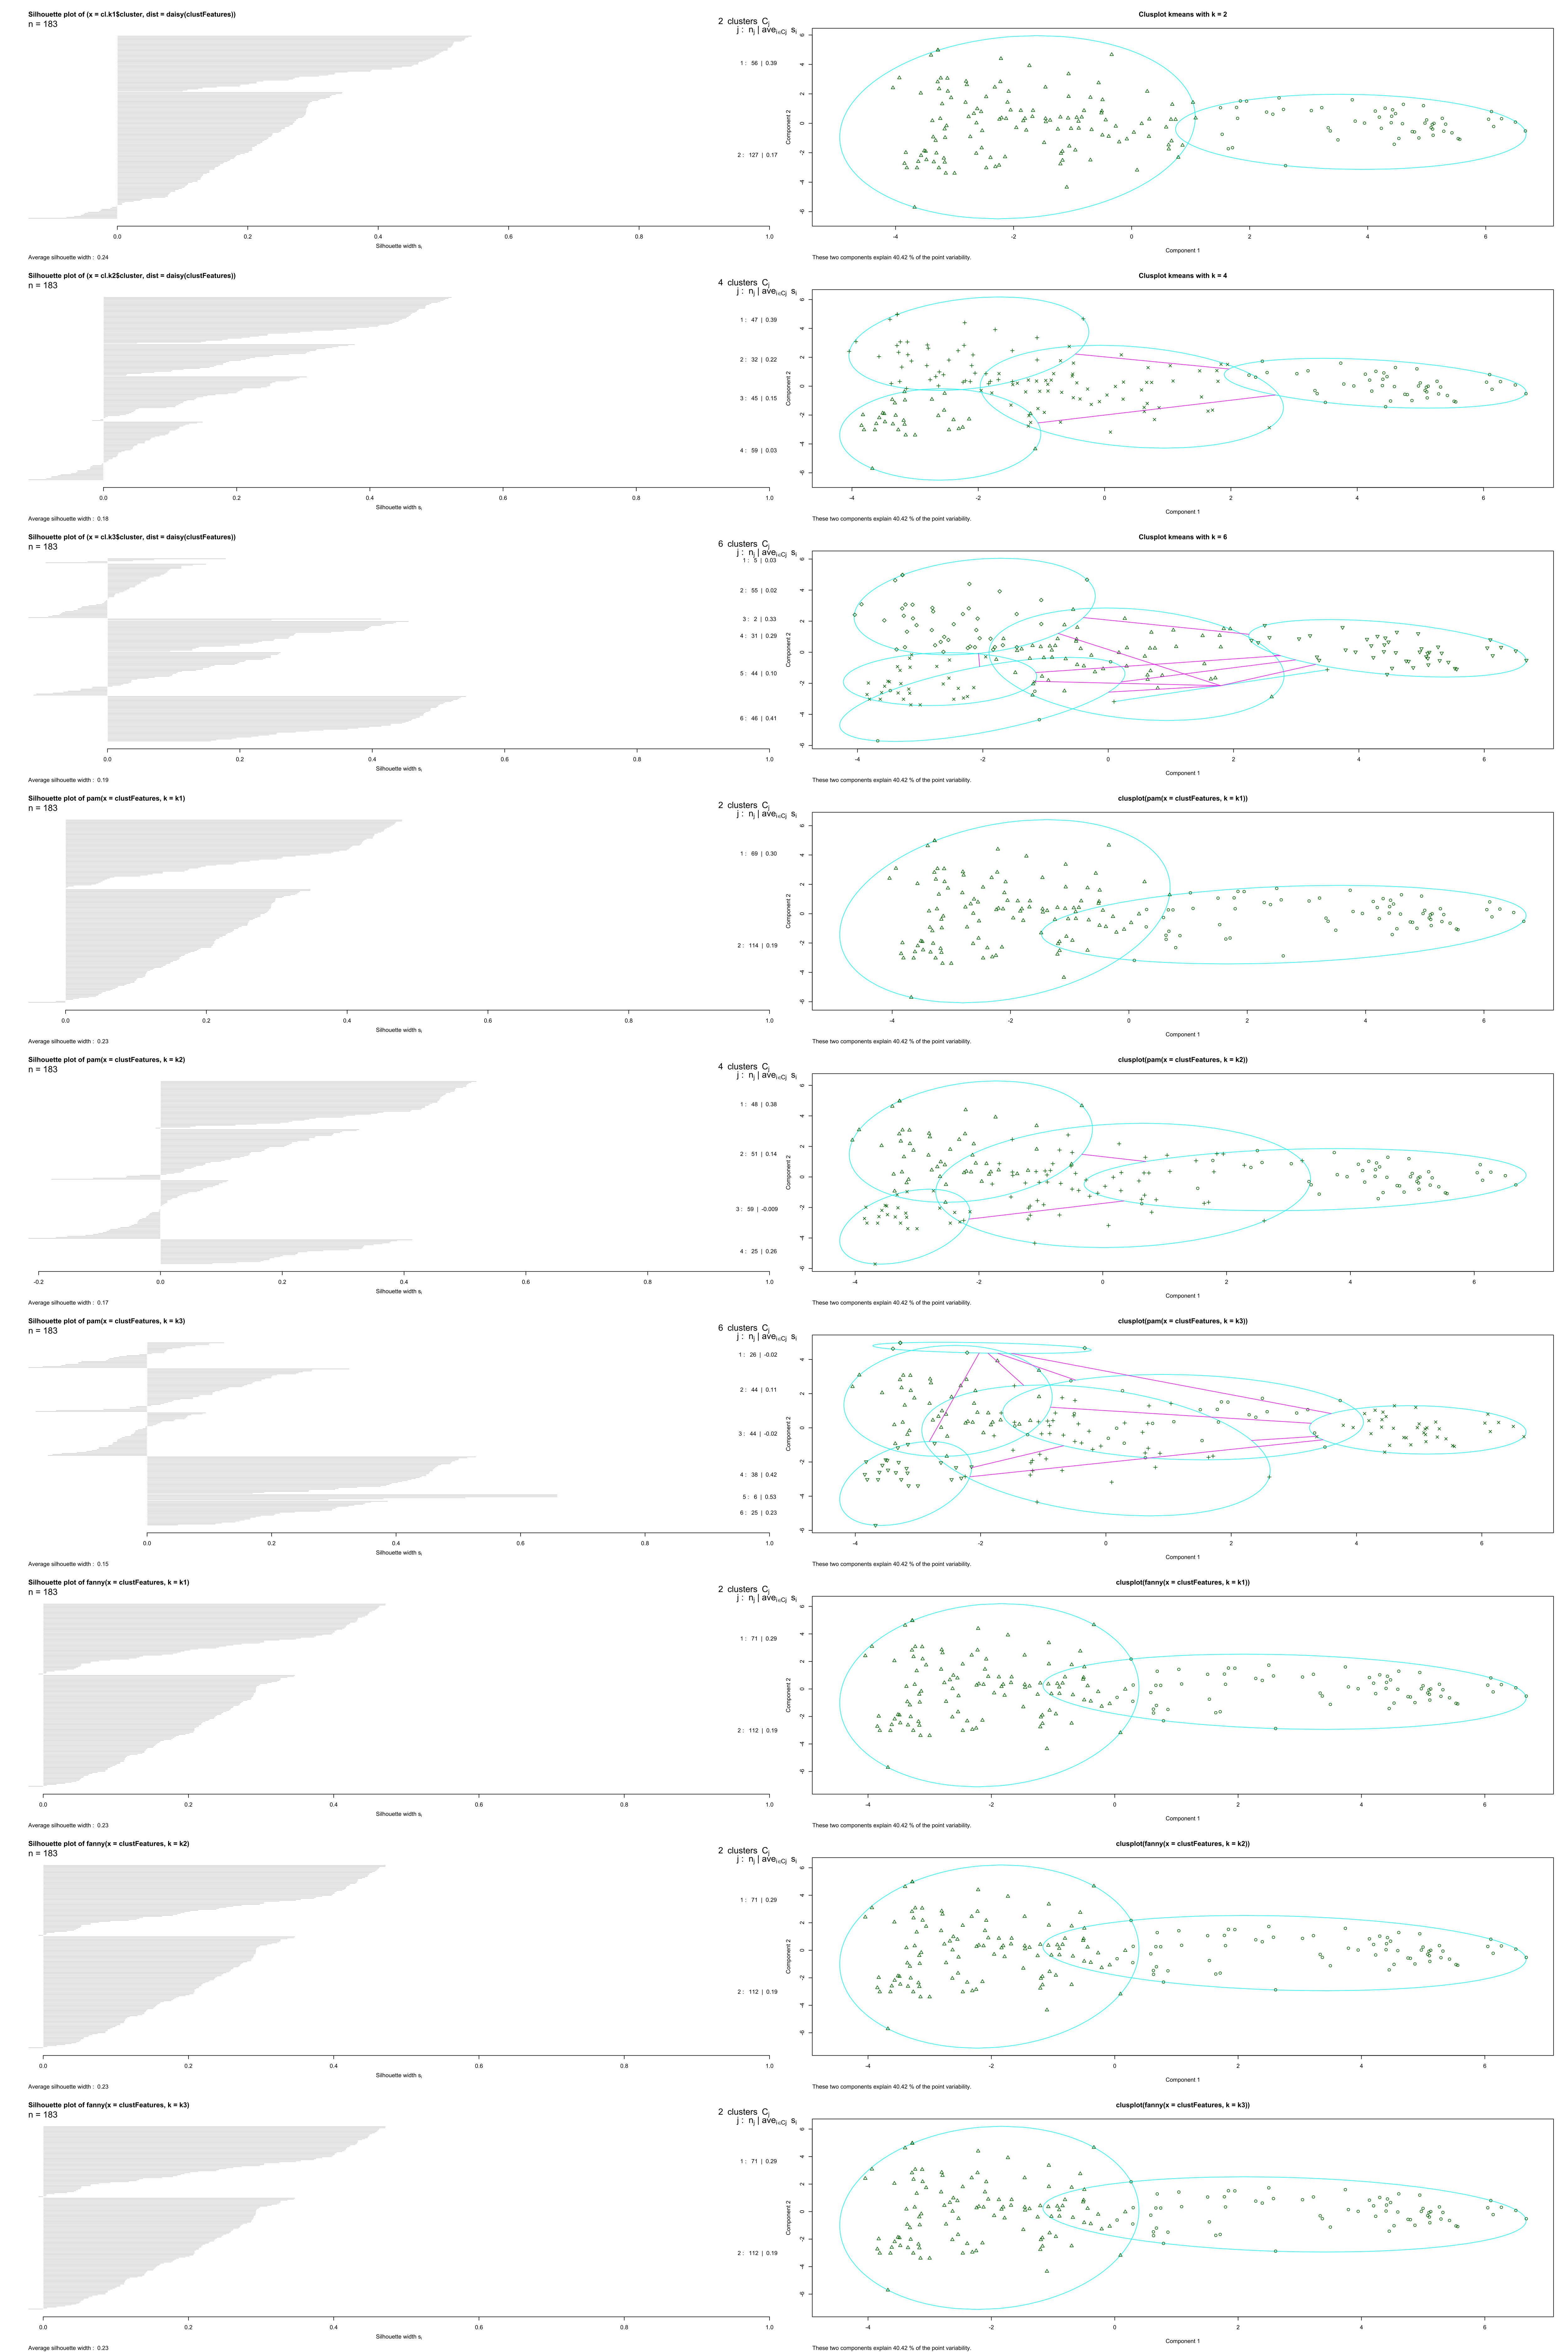
\includegraphics[height=\textheight]{figures/clusteringEvaluationScaled.jpg}
	\caption{Clustering evaluatie met schalen}
	\label{fig:ce}
\end{figure}

 \subsection{Beschrijving clusters}

\begin{figure}[H]
	\centering
	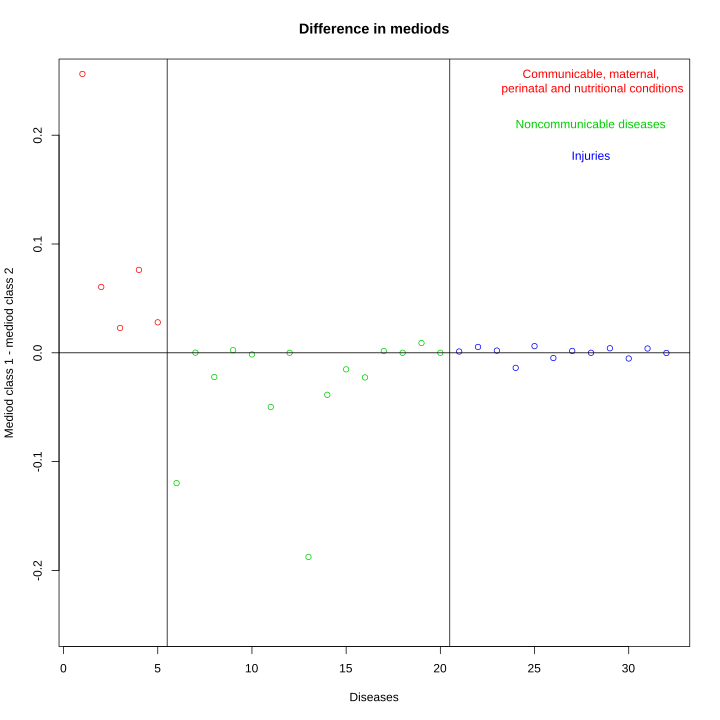
\includegraphics[width=\textwidth]{figures/difMediods.jpg}
	\caption{De verschillen van de gemiddelden}
	\label{fig:dm}
\end{figure}

\subsection{Principaalcomponentenanalyse}
\begin{figure}
	\centering
	\begin{subfigure}{\linewidth}
		\includegraphics[width = .5\linewidth]{figures/PC1vsPC2.png}
		\includegraphics[width = .5\linewidth]{figures/PC1vsPC3.png}
	\end{subfigure}
	\begin{subfigure}{\linewidth}
		\centering

	\end{subfigure}
	\begin{subfigure}{\linewidth}
		\centering
		\includegraphics[width = .5\linewidth]{figures/PC1vsPC4.png}
	\end{subfigure}
	\caption{De eerste principaalcomponent vergeleken met de andere drie belangrijkste principaalcomponenten}
	\label{fig:vglPC}
\end{figure}

 
\end{document}
